% This template is used for pandoc
\documentclass[10pt]{ctexart}

\def\university{Harbin Institute of Technology}
\def\team{Dolls in Pseudo Paradise}
\def\season{2024-2025}

\usepackage{amsmath, amssymb}
\usepackage{booktabs}
\usepackage{graphicx}
\usepackage{float}
\usepackage{comment}
\usepackage[colorlinks, linkcolor = black]{hyperref}

% ==================== Begin     Page ====================
%%%%%% fix pandoc
\providecommand{\tightlist}{\setlength{\itemsep}{0pt}\setlength{\parskip}{0pt}}
\newcommand{\passthrough}[1]{#1}

\usepackage[a4paper, includehead, headsep=0.07in, left=0.45in, right=0.2in, top=0.2in, bottom=0.2in, landscape]{geometry}
\ctexset{
    section = {
        beforeskip = { 0.3ex plus .1ex minus .1ex },
        afterskip  = { 0.1ex plus .1ex }
    },
    subsection = {
        beforeskip = { 0.15ex plus .1ex minus .1ex },
        afterskip  = { 0.1ex plus .1ex }
    },
    subsubsection = {
        beforeskip = { 0.15ex plus .1ex minus .1ex },
        afterskip  = { 0.1ex plus .1ex }
    },
}

% Three columns & landscape to make the code tight
\usepackage{multicol}
\setlength{\columnsep}{25pt}

% ==================== Begin     Font ====================
\usepackage{fontspec}
\setmonofont{FiraCode-Regular.ttf}[
    Path = utils/,
    BoldFont = FiraCode-Bold.ttf,
    ItalicFont = FiraCode-Light.ttf,
    BoldItalicFont = FiraCode-Medium.ttf,
    Contextuals=Alternate           % Activate the calt feature
]

\setCJKmainfont{SourceHanSerif-Regular.otf}[
    Path = utils/,
    BoldFont = SourceHanSans-Regular.otf,
    ItalicFont = SourceHanSerif-Light.otf
]

\newCJKfontfamily[jinwen]\jinwen{DFJinwen-W3}[
    Path = utils/,
    Extension = .otf,
]

% ==================== Begin   Header ====================
\usepackage{fancyhdr}
\usepackage{zref-totpages}
\usepackage{epigraph}
\pagestyle{fancy}
\fancyhf{} % Clear up default styles

\setlength{\headheight}{12.08003pt}

% Header Left: University + team name
\fancyhead[L]{\university -- \textit{\team}}

% Header Center: Section
\fancyhead[C]{\leftmark}

% Header Right: Page number
\fancyhead[R]{Page \thepage\ of \number\numexpr\ztotpages-1\relax}

% Header line
\renewcommand{\headrulewidth}{0.4pt}

%%%%%% Main Content

\usepackage[table]{xcolor}
\usepackage{listings, lstfiracode} % https://ctan.org/pkg/lstfiracode

% Color Palletes from Gihub
\lstset{
  language=[11]C++,
  basicstyle    = \ttfamily\small\color[HTML]{24292E},
  style=FiraCodeStyle,   % Use predefined FiraCodeStyle
  keywordstyle    =\color[HTML]{D73A49}\bfseries,
  commentstyle    =\color[HTML]{6A737D},
  numberstyle     =\color[HTML]{005CC5}\bfseries\sffamily,
  stringstyle     =\color[HTML]{032F62}\bfseries,
  tabsize = 2,
  breaklines,
  basewidth={0.6em, 0.5em},
  breakindent = 1.1em,
  columns = fixed,
  numbers = left,
  frame = single,
  numbersep =5pt,
  framesep  =2pt,
  lineskip  =-1pt,
  mathescape=true
}

% from https://github.com/4thcalabash/code_library/blob/master/tex/format.tex
% an amazing script
% converts an line-number to arbitrary string
\let\othelstnumber=\thelstnumber
\def\createlinenumber#1#2{
    \edef\thelstnumber{%
        \unexpanded{%
            \ifnum#1=\value{lstnumber}\relax
             \tt #2%
            \else}%
        \expandafter\unexpanded\expandafter{\thelstnumber\othelstnumber\fi}%
    }
    \ifx\othelstnumber=\relax\else
      \let\othelstnumber\relax
    \fi
}

% Only 1 and 2 level
\setcounter{tocdepth}{2}

\begin{document}

\begin{titlepage}
    \thispagestyle{empty}

    \vspace*{-1cm}

    \hfill
    \parbox{0.5\textwidth}{
        \epigraph{
            \textsf {Our village of honest men originally consisted of only eight people.} \\
            \textsf {We all picked up and moved to a mountain in the east. Two years of honest and boring daily life passed us by.} \\
            \textsf {One day, one of us found a little hole by a peach tree.} \\
            \textsf {Yes, after that we wandered into this paradise.} \\
            \textsf {And right away, I quit being human.}
        }{\textit{--- Dolls in Pseudo Paradise}}
    }
    \hspace{0.5cm}

    \vfill
    
    \begin{center}
        \Huge {\jinwen 蓬莱人形}算法模板库 \\
        \huge {\textsc{Reference Document} for \textsl{\team}}
    \end{center}

    \vspace*{2cm}

    \begin{figure}[htbp]
        \centering
        \begin{minipage}[c]{0.25\textwidth}
            \centering
            
\includegraphics[width=6cm]{utils/images/hit-logo.png}
        \end{minipage}
        \hspace{1cm}
        \begin{minipage}[c]{0.25\textwidth}
            \centering
            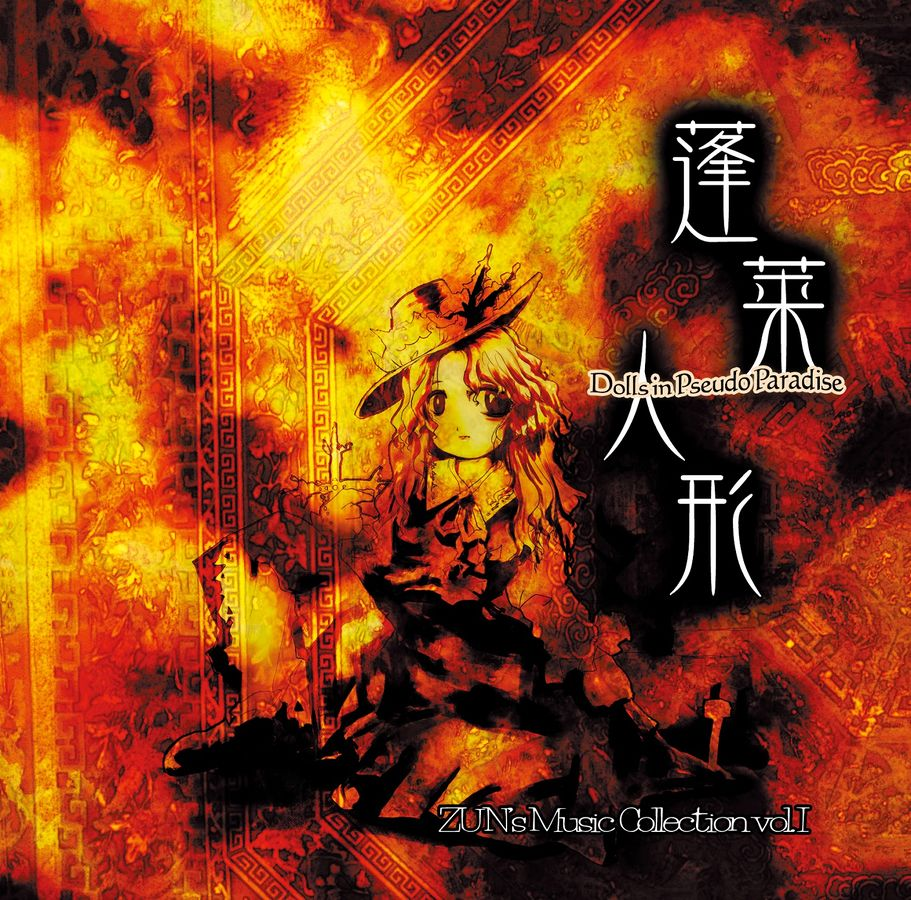
\includegraphics[width=6cm]{utils/images/hourai.jpg}
        \end{minipage}
        \hspace{1cm}
        \begin{minipage}[c]{0.25\textwidth}
            \centering
            
\includegraphics[width=6cm]{utils/images/icpc.png}
        \end{minipage}
    \end{figure}

    \vfill

    \begin{center}
        \Large \color{darkgray} \season \\
        \Large \color{darkgray} \university
    \end{center}

    \vspace*{1cm}
\end{titlepage}

\newpage

\begin{multicols}{3}
    \setcounter{page}{1}

    \tableofcontents
    
    $body$

    \newpage
\end{multicols}

\appendix

\phantomsection
\addcontentsline{toc}{section}{附录}

\def \bangle{\atopwithdelims \langle \rangle}

\begin{table}[H]
	\centering \small \renewcommand\arraystretch{0.8}
	\begin{tabular}{c|c|c|c|c|c|c|c|c|c|c|c|c|c|c|c|c|c|c} \toprule
		$n \leq$ & $10$ & $100$ & $10^{3}$ & $10^{4}$ & $10^{5}$ & $10^{6}$ & $10^{7}$ & $10^{8}$ & $10^{9}$ & $10^{10}$ & $10^{11}$ & $10^{12}$ & $10^{13}$ & $10^{14}$ & $10^{15}$ & $10^{16}$ & $10^{17}$ & $10^{18}$ \\ \midrule
		$\max\omega(n)$ & $2$ & $3$ & $4$ & $5$ & $6$ & $7$ & $8$ & $8$ & $9$ & $10$ & $10$ & $11$ &  $12$ & $12$ & $13$ & $13$ & $14$ & $15$ \\ 
		$\max{d(n)}$ & $4$ & $12$ & $32$ & $64$ & $128$ & $240$ & $ 448$ & $768$ & $1344$ & $2304$ & $4032$ & $6720$ & $10752$ & $17280$ & $26880$ & $41472$ & $64512$ & $103680$ \\ 
		$\pi(n)$ & $4$ & $25$ & $168$ & $1229$ & $9592$ & $78498$ & $664579$ & $5761455$ & $5.08 \mathrm e 7$ & $4.55 \mathrm e 8$ & $4.12 \mathrm e 9$ & $3.7 \mathrm e {10}$ & \multicolumn{6}{c}{$n / \ln(n)$} \\ \midrule
		$n = $ & $2$ & $3$ & $4$ & $5$ & $6$ & $7$ & $8$ & $9$ & $10$ & $11$ & $12$ & $15$ & $20$ & $25$ & $30$ & $40$ & $50$ & $114$ \\ \midrule
		$\log_{10} n$ & $0.301$ & $0.477$ & $0.602$ & $0.698$ & $0.778$ & $0.845$ & $0.903$ & $0.954$ & $1$ & $1.041$ & $1.079$ & $1.176$ & $1.301$ & $1.398$ & $1.477$ \\
		$C(n,n/2)$ & $2$ & $3$ & $6$ & $10$ & $20$ & $35$ & $70$ & $126$ & $252$ & $462$ & $924$ & $6435$ & $184756$ & $5200300$ & $155117520$ \\
		$\mathrm{LCM}(1\dots n)$ & $2$ & $6$ & $12$ & $60$ & $60$ & $420$ & $840$ & $2520$ & $2520$ & $27720$ & $27720$ & $360360$ & $232792560$ & $26771144400$ & $1.444\mathrm e14$ \\ 
		$P_n$ & $2$ & $3$ & $5$ & $7$ & $11$ & $15$ & $22$ & $30$ & $42$ & $56$ & $77$ & $176$ & $627$ & $1958$ & $5604$ & $37338$ & $204226$ & $10^9$ \\ \bottomrule
	\end{tabular}
\end{table}

\tightlist
\begin{itemize}
	\item 质数:$918733, 940649, 923641, 992402371, 903936311, 977499077, 908370375016605079, 973150773996892879, 990191901472122599, 10^{18} + 3$;
	\item NTT 模数:$167772161, 1004535809, 2924438830427668481 = 174310137655 \times 2^{24} + 1$。
\end{itemize}

% 没想好放什么

\end{document}